\documentclass[thesis.tex]{subfiles}

\title{Estimating duration in the presence of misclassification}
\author{Joshua Blake}
\date{\today}

\begin{document}

\ifSubfilesClassLoaded{
  \setcounter{chapter}{5}
}

\chapter{Survival analysis with false negatives} \label{imperf-test}

In \cref{E-perf-test}, a framework for analysing the CIS to produce estimates of the duration of positivity was developed.
However, the initial application of this framework produced an implausibly short estimate.
In this chapter I identify this issue to be the result of false negatives, a form of misclassification bias, within the CIS (\cref{imperf-test:sec:problem}).
I then propose several models of false negatives (\cref{imperf-test:sec:simulate}) and extend the model of \cref{E-perf-test} to incorporate one of them (\cref{imperf-test:sec:modelling})
After showing through simulation that the new model recovers the true duration distribution (\cref{imperf-test:sec:sim-study-results}), I apply it to the CIS data (\cref{imperf-test:sec:application}).
Finally, I discuss the results and further work in \cref{imperf-test:sec:discussion}.

The inclusion of false negatives into survival analysis is an area of much interest, especially in the application of tests for HIV in infants~\autocite[e.g.][]{brownBayesian,balasubramanianEstimation};
\textcite{piresIntervalMisclassify} provide a comprehensive review of approaches.
However, including false negatives with either doubly censored or truncated data has not been addressed.
The situation here requires both.



\section{The problem} \label{imperf-test:sec:problem}

Applying the method of \cref{E-perf-test} to CIS data estimates fewer episodes with a duration of less than three weeks, compared to \cref{E-ATACCC} (see \cref{imperf-test:fig:problem-cis-estimates}).
The \cref{E-ATACCC} estimates are more reliable over the first 2--3 weeks due to them having frequent data collection here (see \cref{E-biology-data:sec:ataccc,E-ATACCC:sec:discussion}).
This suggests an issue in the estimation using CIS data.
\begin{figure}
  \centering 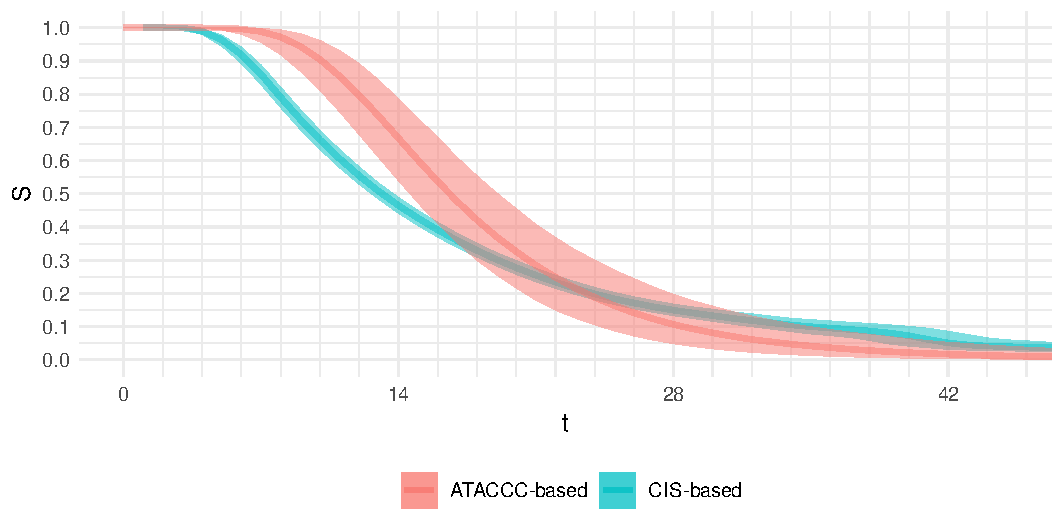
\includegraphics{cis-imperfect-testing/CIS_perfect}
  \caption[Estimating survival using CIS data assuming perfect testing]{Estimates of the survival function using CIS data alongside the ATACCC-based estimates of \cref{E-perf-test}. \label{imperf-test:fig:problem-cis-estimates}}
\end{figure}

Comparing repeated data simulations, using the set-up of \cref{E-perf-test:sec:simulation-study}, to the observed CIS data, suggests that this is due to the high frequency of single positive episodes in the CIS data (compare the histogram with $\psens=1$ and the vertical line in \cref{imperf-test:fig:sim-single-pos}).
A single positive episode is an episode containing exactly one positive test; intuitively, these cause estimates to be shorter because the lower bound on the length of time the episode is 1 day, the shortest possible.
Specifically, if $j$ is a single positive episode then $j$'s admissible region (as defined in \cref{E-perf-test:sec:model}) includes $b_j = e_j = r_j^{(b)} = l_j^{(e)}$.
In this case, the beginning and end day of the episode are both equal to the day of this one positive test.
If this is true, then the duration is $d_j = e_j - b_j + 1 = 1$.
Additionally, short episodes are very likely to be undetected, which means that the design of the CIS cannot rule out many of them occurring.
% This produced the same pattern, that is estimating too many short episodes (not shown).

\Textcite{shenNonparametrica}, generalising \textcite{panNote}, studied the situation when only the terminating event is interval censored (\ie singly censored data) and left truncated.
They showed that the non-parametric maximum likelihood estimator is inconsistent if single positive episodes occur, and the survival function is severely biased downwards.

The CIS is a more complex setting, including double interval censoring and a complex pattern of undetected episodes (see \cref{E-perf-test:sec:problem}).
This means the result cannot simply be extended to the CIS, but still reinforces the intuition that single positive episodes are likely to be problematic.

% Discussion and interrogation of the data led me to
I hypothesised that the reason for the unexpectedly high number of single positive episodes (compared to simulation) was the presence of false negative results.
There are several strands of evidence supporting this hypothesis.
First, it is well known that RT-PCR testing can return false negatives  (see \cref{E-biology-data:sec:PCR}); I explicitly include them in the viral load model of \cref{E-ATACCC}.
Intermittent negatives (described in  \cref{E-biology-data:sec:PCR}) show that they occur within the CIS.
Furthermore, in \cref{imperf-test:sec:simulate}, I expanded the simulation study of \cref{E-perf-test:sec:simulation-study} to include false negatives (see  for more details).
This reproduced the CIS data more faithfully and exhibited the same issues when estimating the duration distribution (see \cref{imperf-test:fig:sim-single-pos}).
\begin{figure}
  \centering 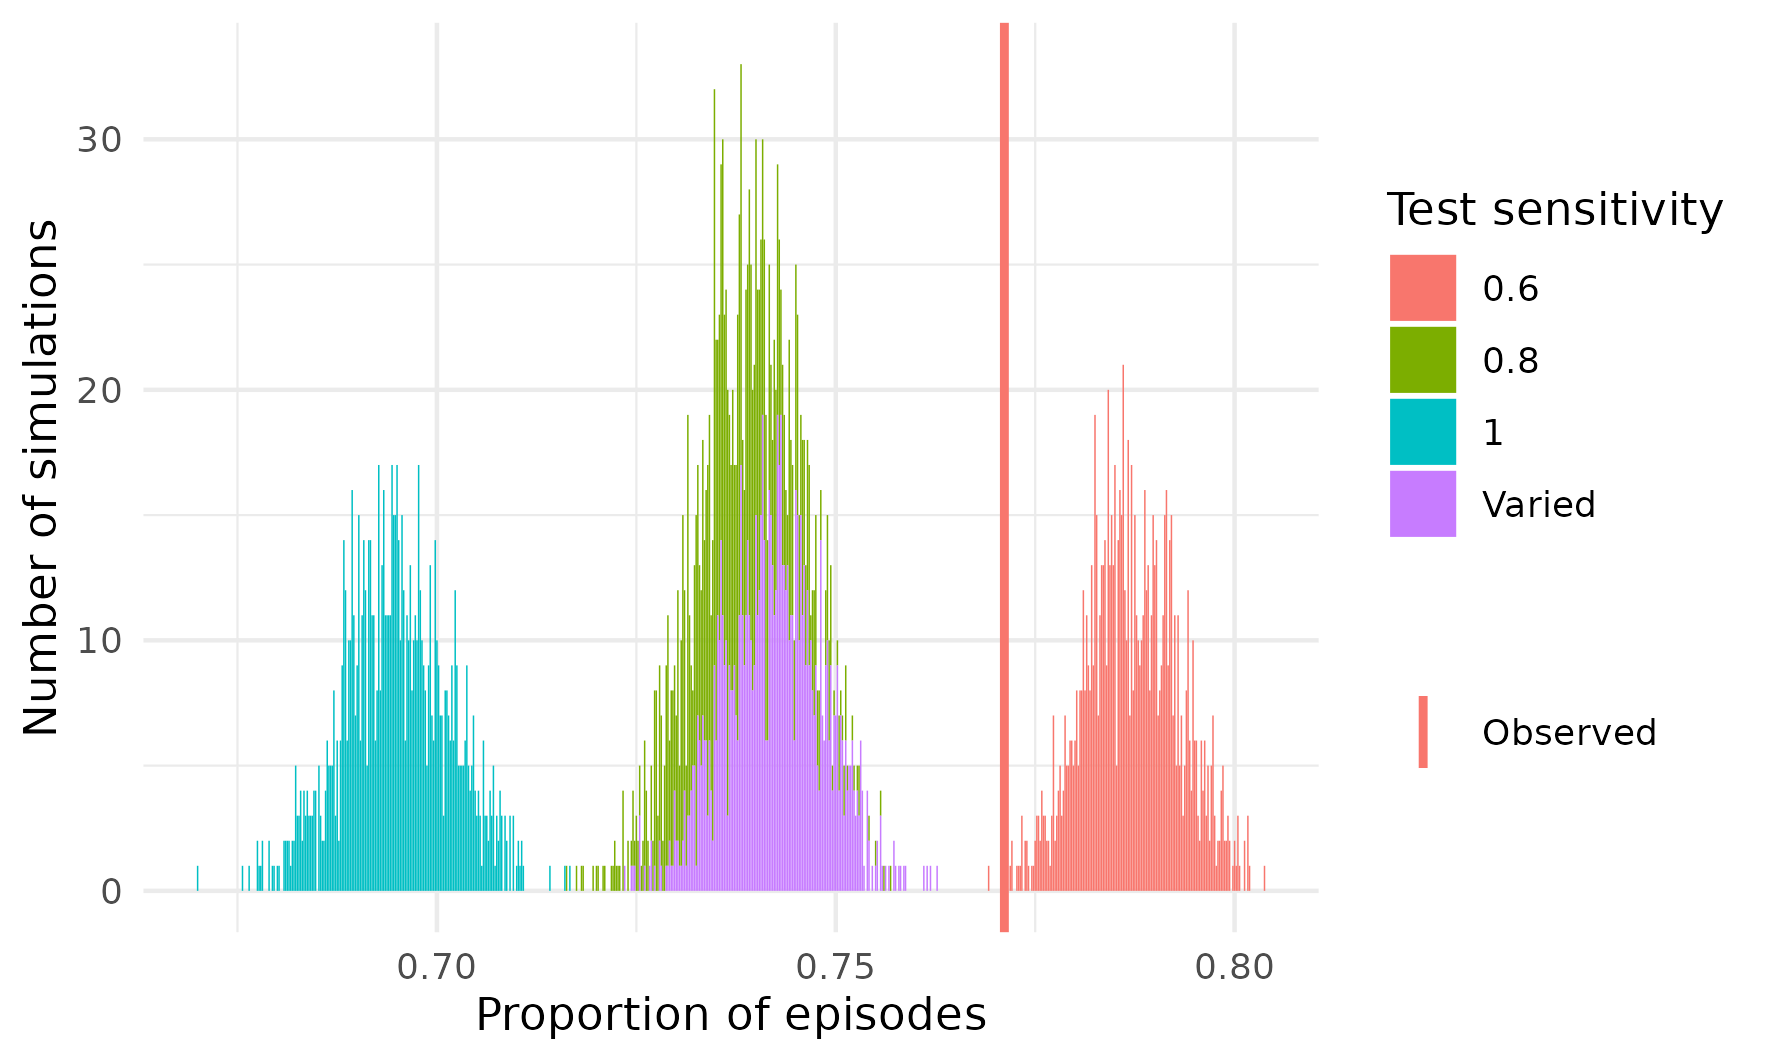
\includegraphics{cis-imperfect-testing/sim-single-positive-episodes}
  \caption[Single positive episodes in CIS simulation]{%
    Proportion of detected episodes which have a single positive episode.
    y-axis is the number of simulations, out of \numprint{1000}, with the indicated proportion.
    Test sensitivity is $\psens$.
    The CIS data is shown as a vertical line.
  }
  \label{imperf-test:fig:sim-single-pos}
\end{figure}

\section{Generative model for false negatives} \label{imperf-test:sec:simulate}

In this section, I introduce a probabilistic model for the generation of false negatives.
The simplest model for false negatives is a constant, non-zero probability of returning a negative test when detectable.
That is the test sensitivity, $\psens$, is less than 1.

Under this model, each test result in a detectable individual is an iid Bernoulli random variable with a probability $\psens$ of producing a positive.
As previously, tests in individuals without ongoing infection episodes are always negative.
I modified the simulation study from \cref{E-perf-test:sec:simulation-study} to generate test results in this way.

Following the modification, more single positive episodes are seen at lower values of $\psens$, with a value between 60\% and 80\% reproducing the number of single positive episodes observed in the CIS data (see \cref{imperf-test:fig:sim-single-pos}).
This is expected: a lower $\psens$ means that multiple positive tests are less likely, and hence the probability of a single positive episode is higher.

In \cref{E-ATACCC}, I estimated that $\psens$ is 95\% (95\% CrI: 93--96\%).
The daily testing this is based on means this is a reliable estimate during the period for which the individuals are followed-up.
The requirement for a much lower value of $\psens$ in the simulation study here suggests this model of false negatives is inadequate.

A better model would be to allow the rate of false negatives to vary over the course of an episode.
False negatives are more likely to occur when the viral load of an individual is low, because there is less virus in their body to sample.
In \cref{E-ATACCC}, this mechanism is incorporated by viewing negative tests as a left-truncation of the observation noise (see \cref{E-ATACCC:sec:observation-modification}).
This observation suggests that a model with a declining test sensitivity as a function of time since infection might be more suitable.

The CIS data provides evidence for a test sensitivity declining over the course of an episode.
\Cref{imperf-test:fig:bounding-cis-sensitivity} demonstrates this by using the following classification for test results.
\begin{enumerate}
    \item All positive results are true positives.
    \item All intermittent negatives are false negatives.
    \item The negative at the end of an episode is a possible false negative.
    \item All other negatives are true negatives.
\end{enumerate}
Here, I am assuming that the probability of two false negative tests at the end of an episode is negligible.
As test sensitivity is the proportion of individuals who should test positive that do so, it can be empirically calculated as number of true positives / (number of true positives + number of false negatives).
Therefore, I calculate the test sensitivity for each day, considering the first positive result in an episode as day 0.
As the latent start day of the infection episode is before the first positive result, day 0 reflects some unknown number of days into the infection episode.
I bound the test sensitivity on each day by assuming either all or none of the possible false negatives (group 3) are in fact false negatives.
% In \cref{imperf-test:fig:bounding-cis-sensitivity} we consider the values produced by assuming the negative following the last positive in an episode could be either a true or false negative as a function of time since the individual was detected (\ie: the first positive test in the episode).
This generates broad bounds, although suggest a declining test sensitivity over the course of an episode (see \cref{imperf-test:fig:bounding-cis-sensitivity}).
Small numbers of tests mean that the series is noisy near the start and the end, such as both bounds being 0 on some days after day 40.
However, the general trend is clear.
\begin{figure}
  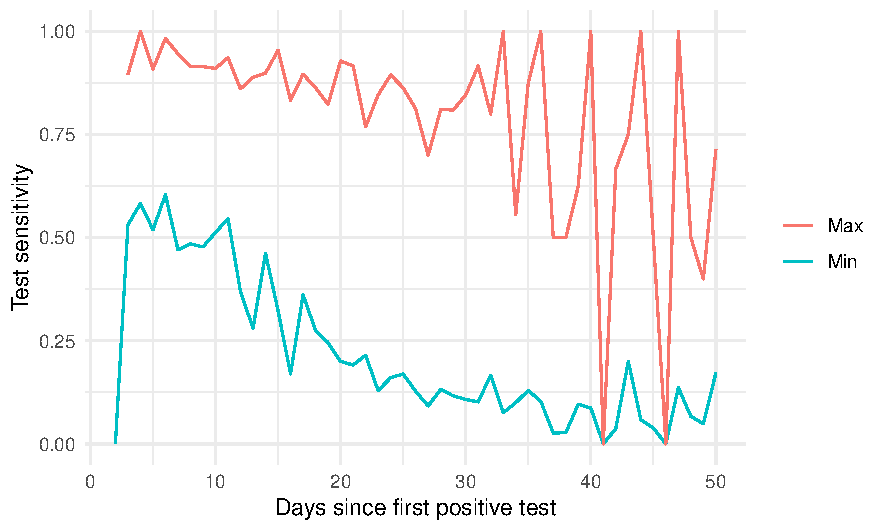
\includegraphics{cis-imperfect-testing/test-sens-bound}
  \caption[Bounding test sensitivity using CIS data]{
    Bounding the test sensitivity using CIS data as a function of time since the infection was detected.
  }
  \label{imperf-test:fig:bounding-cis-sensitivity}
\end{figure}

To assess the sensitivity of the procedure to a time-varying test sensitivity, it will be useful to simulate from a model with a varying test sensitivity as a function of days since the start of the infection episode.
Through consideration of \cref{imperf-test:fig:bounding-cis-sensitivity}, and the interaction of false negatives due to viral load in \cref{E-ATACCC}'s results, I propose the following model.
\begin{equation}
  p_\text{sens}(t) = \begin{cases}
    0.9 - \frac{0.9-0.5}{50}t &t \leq 50 \\
    0.5 &t > 50
  \end{cases}
  \label{imperf-test:eq:variable-test-sensitivity}
\end{equation}
where $t$ is the number of days since infection.
Therefore, this model consists of a linear decline in test sensitivity before a constant minimum point.

I simulate data under this model by, for each test in a detectable individual, calculating $\psens(t-b)$, where $t$ is the day of the test and $b$ is the day the episode began.
The result of the test is then a Bernoulli random variable, independent of all other considerations.
Adapting the simulation study to incorporate this test sensitivity is much more similar to the data (see purple histogram in \cref{imperf-test:fig:sim-single-pos}).
This model does not require low test sensitivities early in the infection, maintaining compatibility with the results in \cref{E-ATACCC}.

\section{Likelihood modification for false negatives} \label{imperf-test:sec:modelling}

In this section, I introduce a simple model of false negatives (\ie allowing $\psens < 1$) into the likelihood derived in \cref{E-perf-test:sec:model}.
The simple model, including a constant test sensitivity, means the likelihood remains tractable.

First, in \cref{imperf-test:sec:modifying-p_ia}, I modify $p_{ia}$, the probability of an episode with test schedule $i$ being admissible, to allow for the episode possibly being longer than observed.
Then, in \cref{imperf-test:sec:modifying-p_iu}, I modify $p_{iu}$, the probability of an episode with test schedule $i$ being undetected, to allow for additional episodes being undetected.

\subsection{Modifying \texorpdfstring{$p_{ia}$}{pia}} \label{imperf-test:sec:modifying-p_ia}

I will modify $p_{ia}$ to allow the negative test following the last positive to be a false negative.
If it is a false negative, then I will consider the episode's end right censored.
However, if it is a true negative, then the episode's end is interval censored, as previously.
A mixture of these scenarios forms the episode's likelihood contribution, with the mixture probability determined by the test sensitivity.

Similar likelihoods have previously appeared in the literature~\autocite[e.g.][eq.\ (2)]{piresIntervalMisclassify}.
However, this prior work was for singly interval censored data; incorporating the double interval censored nature of the CIS data will involve summing over the possible episode start times.

I start by finding the tests that need consideration for episode $j$.
For tractability and simplicity, I consider only tests between the negative tests providing an upper bound on the length of episode $j$.
By definition (see \cref{E-biology-data:sec:cis-episodes}), these are the tests in individual $i(j)$ between $l_j^{(b)} - 1$ and $r_j^{(e)} + 1$ inclusive.

For tractability, assume that the negative test bounding the start of the episode, on day $l_j^{(b)}-1$, is a true negative.
This assumption is reasonable because, since a positive test follows at $r_j^{(b)}$, the negative at $l_j^{(b)}-1$ is likely early in the infection and the test sensitivity is high early in an infection.
Therefore, this is unlikely to be a false negative because, if the individual was detectable at this time, they are in a period with high test sensitivity.
True negatives occur with probability 1, and hence this test does not contribute to the likelihood.

Denote the set of the remaining test times to consider as $\sched'_{i(j)}$.
$\sched'_{i(j)}$ is the set of times individual $i(j)$ was tested between $l_j^{(b)}$ and $r_j^{(e)} + 1$ inclusive.
Denote their results by $\vec{y}_j = \{ y_{i(j)}(t) \ssep t \in \sched'_{i(j)} \}$ where $y_{i(j)}(t) = 1$ if the test on day $t$ in individual $i(j)$ is positive and 0 otherwise.

As I assume that there are no false positives, the infection episode must span at least the period $[r^{(b)}_j, l^{(e)}_j]$, because this period starts and ends with a positive test.
This includes all $t \in \sched'_{i(j)}$ except $t = r_j^{(e)}+1$.
Therefore, the test results $\vec{y}_j$, except the test at $r_j^{(e)}+1$, are either true positives or false negatives.

Consider the negative test at $r_j^{(e)}+1$, the first negative after the start of the episode which may be a false negative.
It is a false negative if and only if the episode ends after the test, \ie $E_j > r_j^{(e)}$.
I proceed by considering whether this is the case and with $B_j = b$ known.

First, if $E_j \leq r_j^{(e)}$, meaning that the test at $r_j^{(e)}+1$ is a true negative and the end of the episode is interval censored as in the previous chapter.
% In this case, the test at $r_j^{(e)} + 1$ is a true negative, as are all other tests not in $\sched'_{i(j)}$.
The true negative occurs with probability 1, by the assumption of no false positives.
\begin{align}
&\prob(\vec{y_j}, E_j \leq r_j^{(e)} \mid B_j = b, p_\text{sens}, \vec{\theta}) \\
&= \prob(\vec{y_j}, l_j^{(e)} \leq E_j \leq r_j^{(e)} \mid B_j = b, p_\text{sens}, \vec{\theta}) \\ % &\text{as no false positives}
&= \prob(\vec{y_j} \mid l_j^{(e)} \leq E_j \leq r_j^{(e)}, B_j = b, p_\text{sens}, \vec{\theta}) \prob(l_j^{(e)} \leq E_j \leq r_j^{(e)} \mid B_j = b, p_\text{sens}, \vec{\theta}) \\
&= \left( \prod_{t \in \sched'_{i(j)}} p_\text{sens}^{y_{i(j)}(t)} (1 - p_\text{sens})^{(1 - y_{i(j)}(t))} \right) \left( S_{\vec{\theta}}(l_j^{(e)} - b + 1) - S_{\vec{\theta}}(r_j^{(e)} - b + 2) \right)
\label{imperf-test:eq:ll-ei-lt-ri}
\end{align}

Second, if $E_j > r_j^{(e)}$.
In this case, the test at $r_j^{(e)}$ is a false negative, occurring with probability $(1 - p_\text{sens})$.
To avoid having to consider tests after $r_j^{(e)}$, which could greatly complicate the likelihood, I model this case as the episode being right censored at $r_j^{(e)}$.
Taking the same approach as before:
\begin{align}
&\prob(\vec{y_j}, E_j > r_j^{(e)} \mid B_j = b, p_\text{sens}, \vec{\theta}) \\
&= \prob(\vec{y_j} \mid E_j > r_j^{(e)}, B_j = b, p_\text{sens}, \vec{\theta}) \prob(E_j > r_j^{(e)} \mid B_j = b, p_\text{sens}, \vec{\theta}) \\
&= \left( \prod_{t \in \sched'_{i(j)}} p_\text{sens}^{y_{i(j)}(t)} (1 - p_\text{sens})^{(1 - y_{i(j)}(t))} \right) (1 - p_\text{sens}) S_{\vec{\theta}}(r_j^{(e)} - b_j + 2)
\label{imperf-test:eq:ll-ei-gt-ri}
\end{align}

These expressions can now be used to form the full replacement for $p_{ia}$, $p'_{ia}$, the likelihood of the data $\vec{y_j}$.
First, augment the data with $b_j$, and split into the cases just discussed:
\begin{align}
p_{ia}'
=& \prob(\vec{y_j} \mid p_\text{sens}, \vec{\theta}) \\
=& \sum_{b = l_j^{(b)}}^{r_j^{(b)}} \left( \prob(\vec{y_j}, E_j \leq r_j^{(e)} \mid B_j = b, p_\text{sens}, \vec{\theta}) + \prob(\vec{y_j}, E_j > r_j^{(e)} \mid B_j = b, p_\text{sens}, \vec{\theta}) \right) \\
  &\times \prob(B_j = b \mid p_\text{sens}, \vec{\theta}).
\intertext{Now, substitute in \cref{imperf-test:eq:ll-ei-lt-ri,imperf-test:eq:ll-ei-gt-ri} and take out the common factor:}
=& \left( \prod_{t \in \sched'_{i(j)}} p_\text{sens}^{y_{i(j)}(t)} (1 - p_\text{sens})^{(1 - y_{i(j)}(t))} \right) \\ & \ \times \sum_{b = l_j^{(b)}}^{r_j^{(b)}} \left( S_{\vec{\theta}}(l_j^{(e)} - b + 1) - S_{\vec{\theta}}(r_j^{(e)} - b + 2) + (1 - p_\text{sens}) S_{\vec{\theta}}(r_j^{(e)} - b + 2) \right) \\ 
  & \times \prob(B_j = b \mid p_\text{sens}, \vec{\theta}) \\
=& \left( \prod_{t \in \sched'_{i(j)}} p_\text{sens}^{y_{i(j)}(t)} (1 - p_\text{sens})^{(1 - y_{i(j)}(t))} \right) \\
  & \times \sum_{b_j = l_j^{(b)}}^{r_j^{(b)}} \left( S_{\vec{\theta}}(l_j^{(e)} - b_j + 1) - p_\text{sens} S_{\vec{\theta}}(r_j^{(e)} - b_j + 2) \right) \\
  & \times \prob(B_j = b \mid p_\text{sens}, \vec{\theta}).
\label{imperf-test:eq:pia-prime}
\end{align}
Note that if $p_\text{sens} = 1$ then $p_{ia}' = p_{ia}$.

If $\psens$ is fixed (\ie has a point prior) and $p(b_j \mid \psens, \vec{\theta}) \propto 1$ (as assumed in \cref{E-perf-test}) then:
\begin{align}
p_{ia}'
&\propto \sum_{b = l_j^{(b)}}^{r_j^{(b)}} S_{\vec{\theta}}(l_j^{(e)} - b_j + 1) - p_\text{sens} S_{\vec{\theta}}(r_j^{(e)} - b + 2).
\label{imperf-test:eq:pia-prime-constant}
\end{align}

\subsection{Modifying \texorpdfstring{$p_{iu}$}{piu}} \label{imperf-test:sec:modifying-p_iu}

Several mechanisms for episodes being undetected were considered when deriving $p_{iu}$ in \cref{E-perf-test:sec:prob-undetected}.
I now consider the additional mechanisms arising due to false negatives.
Specifically, episode $j$ could be undetected if the first test after $b_j$ is a false negative and then there are no subsequent positive tests.

This false negative would occur at the first test after the infection episode begins, on day $b_j + \tau_{\sched_{i(j)}}(b_j)$ (see \cref{E-perf-test:sec:prob-undetected}).
A false negative occurring requires that the episode has not yet ended but a negative still occurs.
The episode has not yet ended at the time of the test if $e_j = b_j + d_j - 1$ is after the test, that is the duration of the infection $d_j > \tau_{\sched_{i(j)}}(b_j)$.
Conditional on the episode having not yet ended, the test result is negative with probability $1 - \psens$.

For there to be no subsequent positive tests, all tests up until day $e_j$ are false negatives.
I assume there is a negligible probability of two false negatives.
Therefore, this can only occur if the episode ends before another test.
Denote the number of days between $b_j$ and the test following the false negative as $\tau^2_{\sched_{i(j)}}(b_j) \stackrel{\text{def}}{=} \tau_{\sched_{i(j)}}(\tau_{\sched_{i(j)}}(b_j) + 1)$.
Then, the episode ends before this test if $d_j < \tau^2_{\sched_{i(j)}}(b_j)$.

Therefore, this mechanism causes episode $j$ to be undetected if all the following conditions hold.
\begin{enumerate}
    \item The episode would have been detected considering only the mechanisms in \cref{E-perf-test:sec:prob-undetected}. That is $b_j > \min(\sched_{i(j)})$ and $e_j \geq \tau_{\sched_{i(j)}}(b_j) + b_j$.
    \item The episode ends in the interval $[\tau_{\sched_{i(j)}}(b_j) + b_j, \tau^2_{\sched_{i(j)}}(b_j) + b_j]$.
      Note that the lower bound here is exactly the bound on $e_j$ in the previous condition.
      Equivalently, $\tau_{\sched_{i(j)}}(b_j) + 1 \leq d_j \leq \tau^2_{\sched_{i(j)}}(b_j) + 1$.
    \item A false negative occurs on day $\tau_{\sched_{i(j)}}(b_j) + b_j$. Conditional on the previous condition, this occurs with probability $1 - \psens$.
\end{enumerate}

The probability of this occurring, conditional on $B_j = b_j > \min(\sched_{i(j)})$ is:
\begin{align}
&\prob \left(
    \tau_{\sched_{i(j)}}(b_j) + 1 \leq D_j \leq \tau^2_{\sched_{i(j)}}(b_j) + 1
    \mid B_j = b, \vec{\theta} \right) (1 - \psens) \\
&= \left( S_{\vec{\theta}}(\tau_{\sched_{i(j)}}(b_j) + 1) - S_{\vec{\theta}}(\tau^2_{\sched_{i(j)}}(b_j) + 1) \right) (1 - \psens).
\end{align}
Summing over $b_j$ for $\min \sched_{i(j)} < b_j \leq T$ ($T$ being the last day of the period considered), in the same way as \cref{perf-test:eq:piu}, gives:
\begin{align}
\zeta = (1 - p_\text{sens})\frac{1}{T} \sum_{b=\min(\sched_{i(j)}) + 1}^T \left( S_{\vec{\theta}}(\tau_{\sched_{i(j)}}(b) + 1) - S_{\vec{\theta}}(\tau^2_{\sched_{i(j)}}(b) + 1) \right).
\end{align}

Denote the replacement for $p_{iu}$ as $p_{iu}'$.
$p_{iu}'$ is the probability of episode $i$ being undetected, considering both the mechanisms from \cref{E-perf-test} and the new mechanism here.
These mechanisms are mutually exclusive.
Hence, $p_{iu}'$ is the sum of these, $p_{iu}' = p_{iu} + \zeta$.
For the posterior density, \cref{E-perf-test:eq:full-posterior}, $1 - p_{iu}'$ is the required quantity.
\begin{align}
1 - p_{iu}'
&= 1 - p_{iu} - \zeta \\
&= \frac{1}{T} \sum_{b=\min(\sched_{i(j)}) + 1}^T \left( p_\text{sens} S_{\vec{\theta}}(\tau_{\sched_{i(j)}}(b) + 1) + (1 - p_\text{sens}) S_{\vec{\theta}}(\tau^2_{\sched_{i(j)}}(b) + 1)\right).
\label{imperf-test:eq:pit-prime}
\end{align}

$p_{iu}'$ and $p_{ia}'$ are substituted for $p_{iu}$ and $p_{ia}$ respectively in \cref{E-perf-test:eq:full-posterior}.
The posterior density is otherwise unchanged.

\section{Simulation study} \label{imperf-test:sec:sim-study-results}

Here, I modify the simulation study in \cref{E-perf-test:sec:simulation-study} to assess several features of the statistical model I proposed in the previous section.
First, the ability to identify the survival function even with false negatives.
Second, the impact of misspecifying $\psens$, such as the assumption that it is constant.
Finally, the impact of the simplifying assumptions made in \cref{imperf-test:sec:modelling} for tractability.
These assumptions are that the negative at $l^{(b)}_j - 1$ is a true negative and that there is a negligible probability of missing an episode due to two false negatives.

I simulate datasets under four conditions: a constant $\psens$ of 0.6, 0.8, or 1.0 (the latter being the same as the simulated data in \cref{E-perf-test:sec:simulation-study}), or the varying test sensitivity model proposed at the end of \cref{imperf-test:sec:simulate}.
The simulation is otherwise unchanged from that in \cref{E-perf-test:sec:simulation-study}.
The number of single positive episodes in each of these conditions, compared to the number observed in the CIS data, is shown in \cref{imperf-test:fig:sim-single-pos}.

For each simulated dataset, I estimate the survival function using the likelihood proposed in \cref{imperf-test:sec:modelling} and assuming $\psens$ equals 0.6, 0.8, or 1.0.
If the dataset was simulated using a constant $\psens$, and that value of $\psens$ matches the value assumed during inference, I refer to $\psens$ as being correctly specified; otherwise, I refer to it as misspecified.
However, there is still some misspecification of the model to false negatives owing to the simplifying assumptions made.
The amount that the simplifying assumptions are violated increases as $\psens$ decreases.

I use either the independent (vague) or model combination priors for the survival (described in \cref{E-perf-test:sec:parameters-priors}).
These were shown to be the best performing priors in \cref{E-perf-test:sec:results}.
Therefore, there are a total of 24 possible scenarios, although not all are shown.
These are each combination of: 4 simulated datasets, with varying $\psens$; 3 values of $\psens$ in inference; and 2 priors for the hazard.

When $\psens = 0.8$ and is correctly specified, the model recovers the true survival time well (see \cref{imperf-test:fig:constant-test-sensitivity}(B)).
The informative prior, in comparison to the vague prior, helps to overcome the misspecification due to the simplifying assumptions, moving the estimated survival function closer to its true survival time.
However, when $\psens = 0.6$, this is no longer the case (see \cref{imperf-test:fig:constant-test-sensitivity}(A)).
This is likely caused by too large a violation of the simplifying assumptions made in \cref{imperf-test:sec:modelling}.
\begin{figure}
  % \makebox[\textwidth][c]{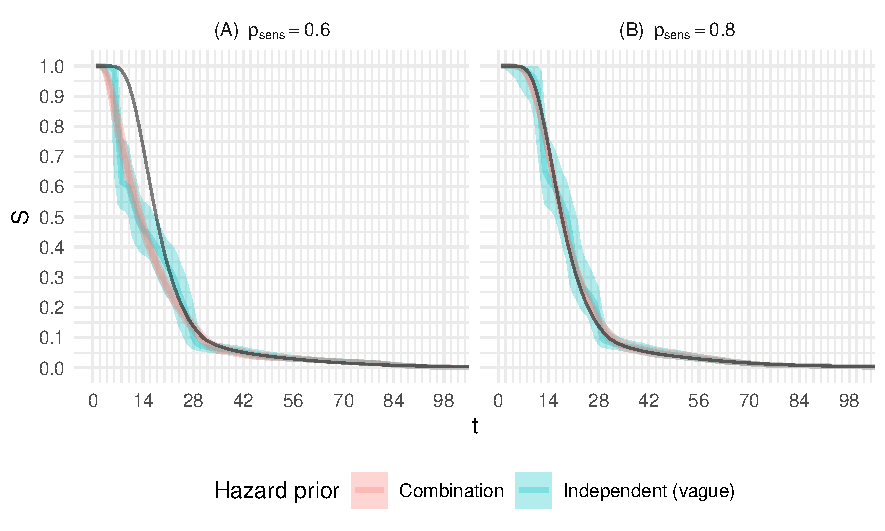
\includegraphics[width=1.2\textwidth]{cis-imperfect-testing/sim-constant-sensitivity}}
  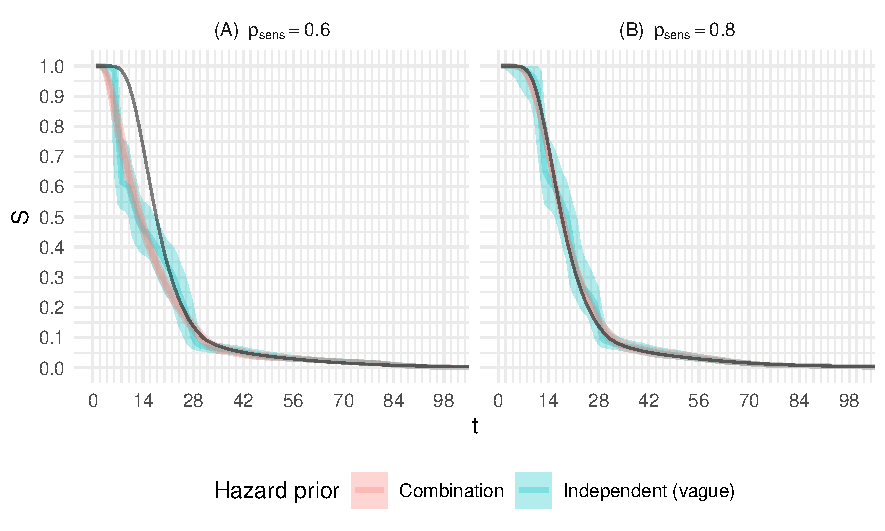
\includegraphics[width=\textwidth]{cis-imperfect-testing/sim-constant-sensitivity}
  \caption[Simulation study results with constant test sensitivity]{%
    Posterior (median and 95\% credible interval) of the survival time for the simulation study with a correctly specified test sensitivity.
    The true survival time is shown in black
  }
  \label{imperf-test:fig:constant-test-sensitivity}
\end{figure}

Next, I considered the consequence of $\psens$ being misspecified, I use the model combination prior because it is the better performing prior in the correctly specified case.
If the test sensitivity is misspecified, that is the assumed value for $p_\text{sens}$ in \cref{imperf-test:eq:pit-prime,imperf-test:eq:pit-prime} is different to the value used in the simulation, then the survival time will be biased (see \cref{imperf-test:fig:misspecified-test-sensitivity}).
If $\psens$ is misspecified and too low (see \cref{imperf-test:fig:misspecified-test-sensitivity}(A)), then the posterior estimate initially follows the true value but then separates.
The number of episodes inferred to have truly ended by the first negative is too high, and hence the survival time is overestimated.
This effect dominates over the opposing bias of overestimating the number of undetected episodes.
The opposite occurs if the test sensitivity is assumed to be too high, although the posterior moves away from the truth earlier (see \cref{imperf-test:fig:misspecified-test-sensitivity}(C)).
\begin{figure}
  % \makebox[\textwidth][c]{
    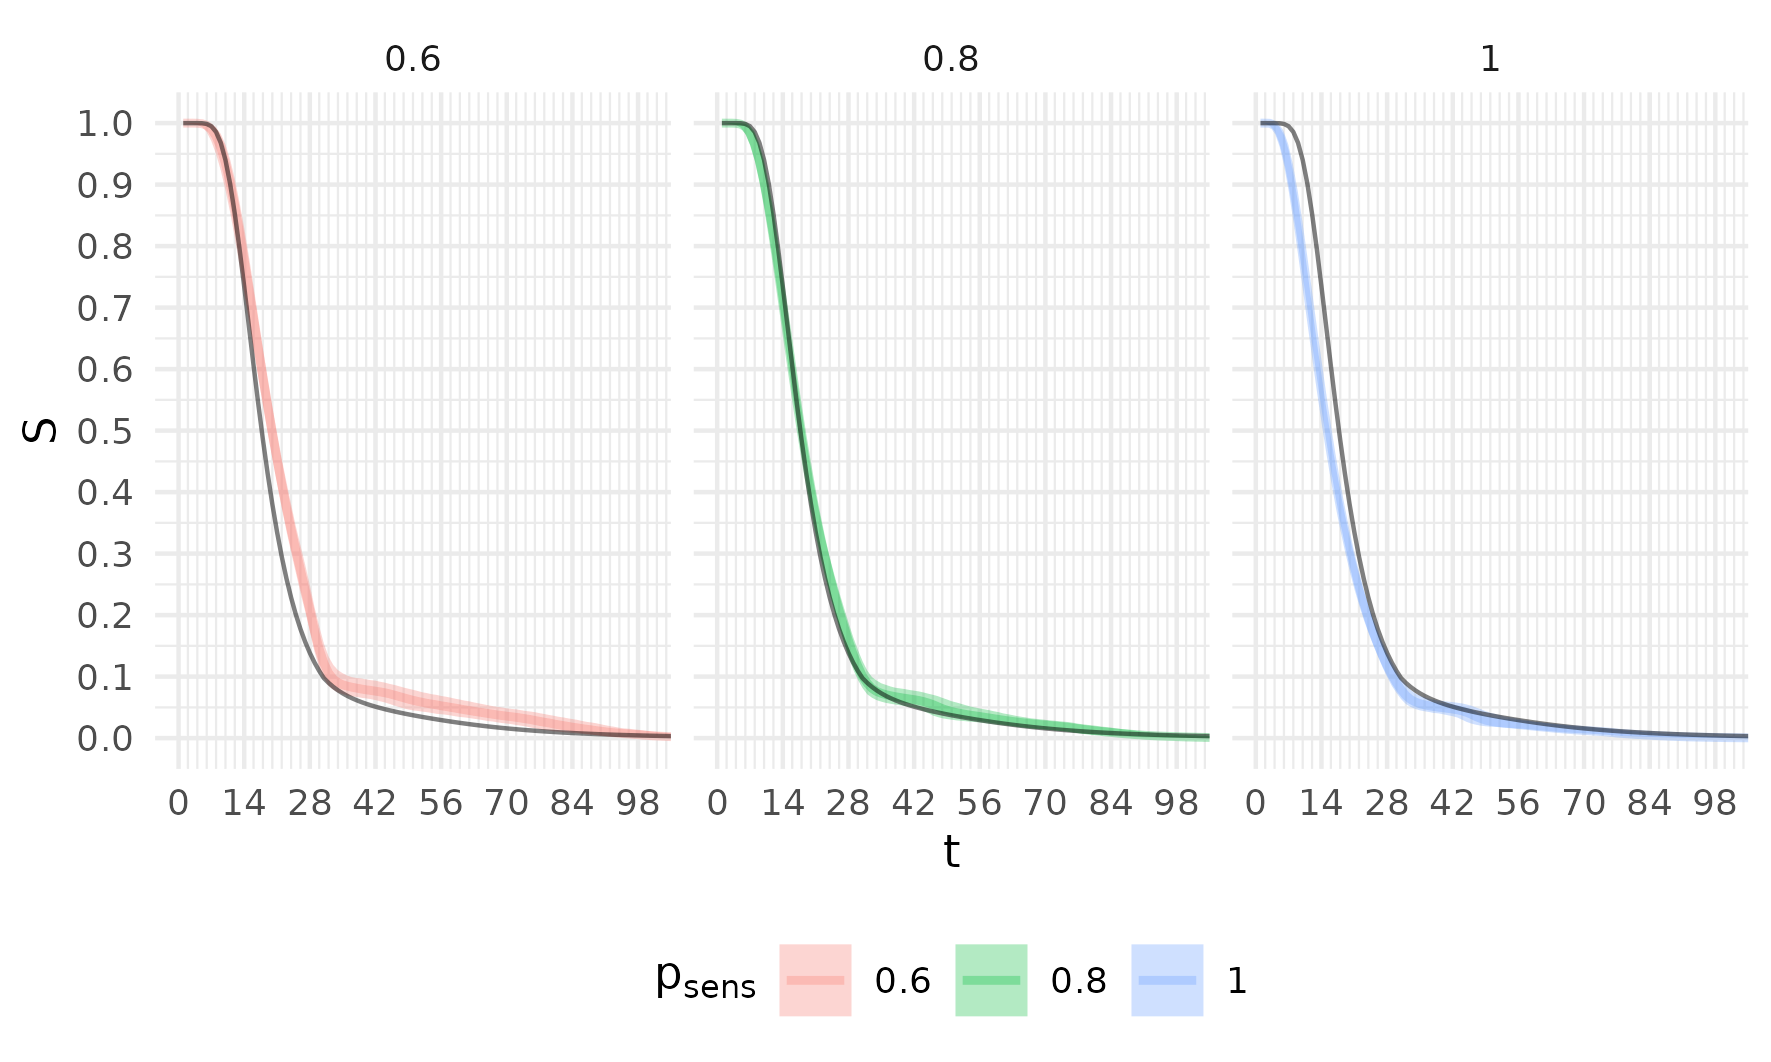
\includegraphics[width=\textwidth]{cis-imperfect-testing/sim-misspecified-sensitivity}
  \caption[Simulation study results with misspecified test sensitivity]{%
    Posterior (median and 95\% credible interval) of the survival time for the simulation study with a possibly misspecified test sensitivity.
    The true survival time is shown in black
    All simulations use a constant test sensitivity of 0.8, but the inference procedure assumes different values, as per the key.
    Hence, (B) is correctly specified but (A) and (C) have misspecified $\psens$.
  }
  \label{imperf-test:fig:misspecified-test-sensitivity}
\end{figure}

The results when a varying test sensitivity (\cref{imperf-test:eq:variable-test-sensitivity}) is used for the simulation are similar to a constant 0.8 test sensitivity (see \cref{imperf-test:fig:variable-test-sensitivity}).
This suggests that the simplified model, with constant test sensitivity, is sufficient for recovering the true survival time.
Estimating the test sensitivity is not possible without a more complex model, as discussed in \cref{imperf-test:sec:discussion}.
Therefore, I will apply this model to the real CIS data in the next section.
\begin{figure}
  % \makebox[\textwidth][c]{
    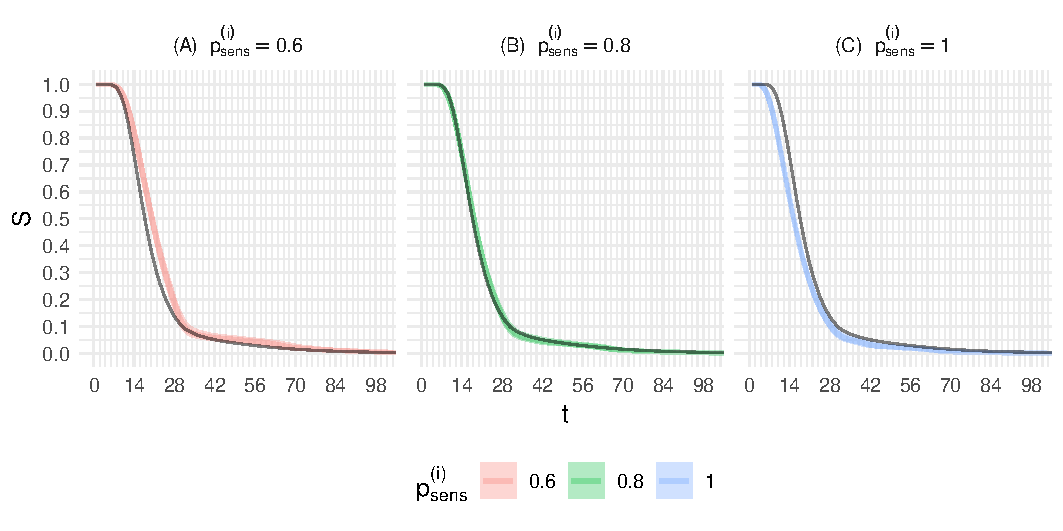
\includegraphics[width=\textwidth]{cis-imperfect-testing/sim-variable-sensitivity}
  \caption[Simulation study results with varying test sensitivity]{%
    Posterior (median and 95\% credible interval) of the survival time for the simulation study with a variable test sensitivity.
    Each panel shows the results of performing inference with a different assumed value for the test sensitivity.
    The posterior estimate using a model with a constant test sensitivity of 0.8 (B) is similar to the true value (black line).
  }
  \label{imperf-test:fig:variable-test-sensitivity}
\end{figure}

\section{Application to CIS data} \label{imperf-test:sec:application}

In this section I apply the approach described in this chapter to the CIS episodes dataset I described in \cref{perf-test:sec:data-notation}.
This is the \numprint{4800} CIS infection episodes first detected between 10 Oct 2020 and 6 Dec 2020 inclusive and have negatives bounding the start and end time of the episode.

Unlike in the simulation studies, an uninformative prior on $\ntot$ led to implausible estimates of the duration distribution.
The uninformative prior led to high posterior estimates of $\ntot$, and hence an implausibly large number of episodes with durations of less than five days.
Therefore, I based an informative prior for $\ntot$, $\ntot \sim \NBc(\mu, r)$ (as in \cref{E-perf-test:sec:model}, see \cref{E-distributions} for definition), using pre-existing estimates of the total number of infections to give $\mu\inform$ and $r\inform$.
\Textcite{birrellRTM2} estimated the total number of infections in England over the time period I consider, with posterior mean \numprint{4136368} and standard deviation \numprint{27932}.
% This model gives a posterior mean of \numprint{4136368} cumulative infections in England in the time period I consider, with a posterior standard deviation of \numprint{27932}~\citePersonalComms{Paul Birrell}.
\todo{Insert correct citation for RTM paper 2 once available}
Approximating this distribution as a negative binomial and scaling the mean to the size of the CIS cohort gives the prior $\mu\inform = \numprint{25132}$ and $r\inform = \numprint{22047}$.

With this prior, the model produces plausible estimates of the duration distribution (see \cref{imperf-test:fig:cis-estimates}).
This estimate (blue) has more long episodes than the estimate in \cref{E-ATACCC} (red).

The qualitative increase in long episodes is robust to the choice of prior for $\ntot$, the assumed value for $\psens$ (see \cref{imperf-test:fig:cis-sensitivity}), and the choice of prior for the hazards, $\lambda_t$ (see \cref{E-perf-test:sec:parameters-priors}).
However, the survival proportion over the first 4 weeks is sensitive to these choices.
The estimate using a test sensitivity of 0.8 and $\NBc(\mu\inform, r\inform)$ give a median survival time most similar to that of \cref{E-ATACCC}.
\begin{figure}
  \centering 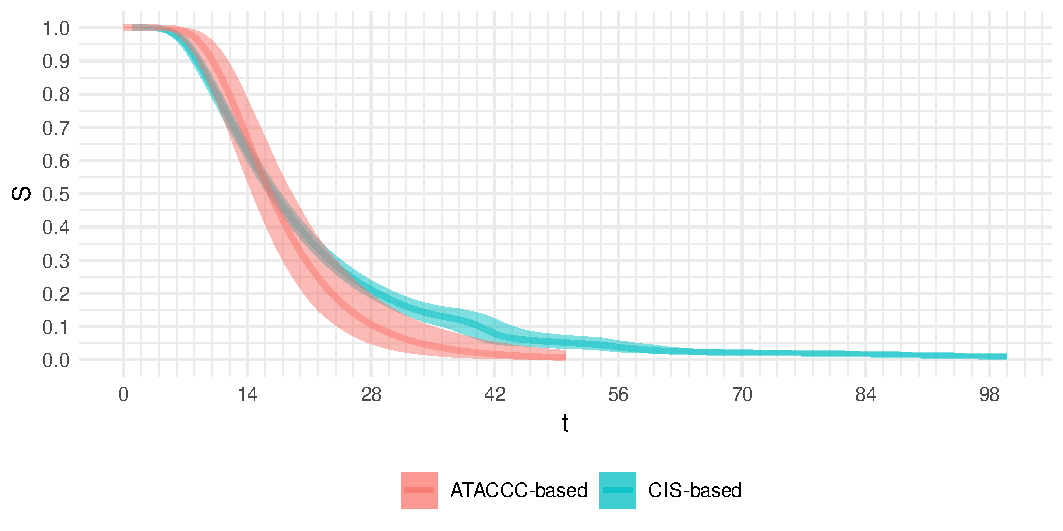
\includegraphics{cis-imperfect-testing/CIS_final}
  \caption{Duration estimates using CIS and ATACCC data.}
  \label{imperf-test:fig:cis-estimates}
\end{figure}
\begin{figure}
  \thisfloatpagestyle{empty}
  \makebox[\textwidth][c]{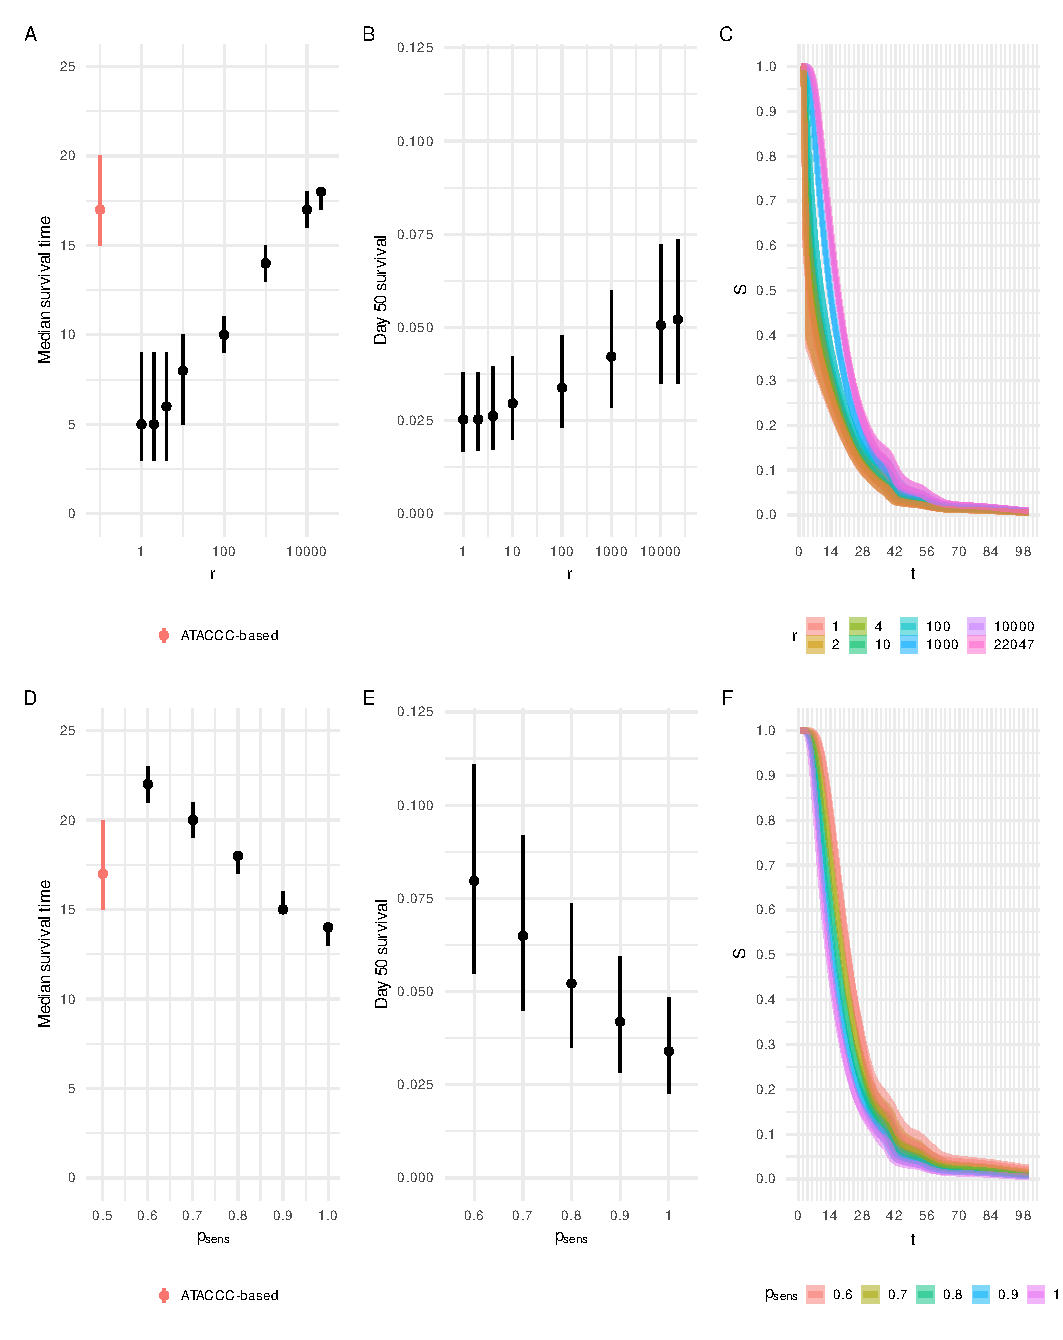
\includegraphics{cis-imperfect-testing/CIS_vary}}
  \caption[Sensitivity of CIS estimates to the prior.]{%
    (A-C) Sensitivity of CIS estimates to the value of $r$, the dispersion of the prior for $\ntot$ (a larger $r$ means a more informative prior) when $\psens = 0.8$.
    (D-F) Sensitivity of CIS estimates to the value of $\psens$ when $r = r\inform$.
    A and D: median survival time, in comparison to the ATACCC-based estimate of \cref{E-ATACCC} (shown in red).
    B and E: survival at day 50, $S_{\vec{\theta}}(50)$.
    C and F: full survival curves out to day 100.
  }
  \label{imperf-test:fig:cis-sensitivity}
  \todo[inline]{Optional improvement: Could highlight the "preferred" model which exists in both rows and is the one used subsequently, and/or include ATACCC in the far-right hand column}
\end{figure}

The estimates are most sensitive to the choice of $r$, the strength of the prior on $\ntot$.
A very weak, almost uninformative, prior on this quantity causes the posterior estimate to be much higher than the estimate from \textcite{birrellRTM2}.
When increasing the prior's strength, the posterior estimate moves towards the prior smoothly, as expected (see \cref{imperf-test:fig:ntot}).
As discussed previously, the \cref{E-ATACCC} estimates are reliable for the first 2--3 weeks, notably including the median time.
The median using $r\inform$ matched \cref{E-ATACCC}'s median estimate and is a principled choice because it is based directly on the prior work \textcite{birrellRTM2}.
Therefore, I use this estimate in the application to the CIS data.
\begin{figure}
  \centering 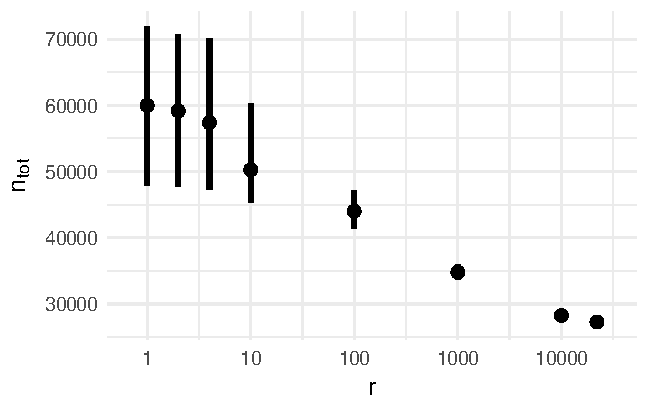
\includegraphics{cis-imperfect-testing/CIS_ntot}
  \caption[Sensitivity of estimates of $\ntot$ to the prior.]{How the posterior estimate of $\ntot$ changes with the value of $r$ in the prior on $\ntot$.}
  \label{imperf-test:fig:ntot}
\end{figure}

\section{Discussion} \label{imperf-test:sec:discussion}

In this chapter, I developed a novel method to incorporate false negatives into the survival analysis of \cref{E-perf-test}.
I then applied this method to the CIS data, estimating the tail of the duration distribution without the strong model assumptions and extrapolation in \cref{E-ATACCC}.
The qualitative features of the estimated distribution are robust to the assumed value for $\psens$, and the choice of prior for $\lambda$, although the quantitative details are not.
The estimates of the tail, the primary purpose of this chapter, are in addition somewhat robust to the choice of prior for $\ntot$.
However, the rest of the distribution is sensitive to this choice.

An informative prior on $\ntot$ is required is for the bulk of the distribution to agree with those in \cref{E-ATACCC} and the wider literature.
In the simulation study, the uninformative prior on $\ntot$ performed well, even when the test sensitivity was misspecified.
A possible explanation is that the true changes in the test sensitivity is significantly different to the function in \cref{imperf-test:eq:variable-test-sensitivity}.
In particular, the test sensitivity for long episodes may become much lower than 50\%.
This allows many more episodes to be undetected than the model assumes, and hence a higher $\ntot$ is required to explain the data.
Furthermore, it violates assumptions made in \cref{imperf-test:sec:modelling}; this is similar to when the simulating using a too low test sensitivity.
Violating these assumptions would lead to unpredictable inference results, perhaps those seen here.

Ideally, the test sensitivity would be estimated from the data.
However, this would require incorporating time-varying test sensitivity into the likelihood.
If the current model, with a constant $\psens$, is used then the estimate of $\psens$ would be heavily informed be intermittent negatives (the first, constant term in \cref{imperf-test:eq:pia-prime}).
These negatives will, in general, be further from the end of an episode than a randomly selected test.
Therefore, considering the viral dynamics from \cref{E-ATACCC}, the viral load will be higher and false negatives rarer.

Estimating the test sensitivity excluding intermittent negatives is not possible because \cref{imperf-test:eq:pia-prime-constant,imperf-test:eq:pit-prime} are both monotonically decreasing in $\psens$; therefore, the likelihood always favours $\psens = 0$ (\ie no true positives).
This aligns with the situation with singly interval censored, untruncated data, when stopping at the first observed time of the terminating event (which may be misclassified) means that the test sensitivity cannot be estimated~\autocite[e.g.]{titmanMisclassify}.

Estimating a time-varying $\psens$ with $S_{\vec{\theta}}$ jointly may cause identifiability issues.
Previous studies have avoided issues by including external information (such as a prior giving the magnitude) on $\psens$, or test results from later follow-up~\autocite[and references therein]{piresIntervalMisclassify}.
However, these studies use a constant $\psens$.
Whether these methods are sufficient for the model to be identifiable with a time-varying $\psens$ needs further investigation.
A simple parametric form of the test sensitivity, such as that proposed by \textcite{brownBayesian}, may be sufficient to allow identifiability.
In any case, the likelihood, especially $p_{iu}'$, would be substantially complicated by such an addition which may greatly increase the computational cost of inference.

The assumption, made in \cref{E-perf-test}, was that the episode start times are independent.
However, because infections are the result of a counting process with intensity shared between individuals (see \cref{E-inc-prev:sec:infection-process}), this assumption is violated.
Prevalence was fairly constant over the period I chose, suggesting the same is true of the incidence.
Additionally, some simulations exploring the results of changing incidence suggested this would not have a large effect on the results (not shown).

% However, comparing the CIS and simulated datasets do not show any differences which suggest what in the data is causing these differences.
% Then, the additional undetected infections implied by a 
% This would lead to more undetected infections than the model assumes, and hence a higher $\ntot$ is required to explain the data.

\section{Conclusion} \label{imperf-test:sec:conclusion}

In this chapter, I developed and applied novel methodology to estimate the duration distribution of RT-PCR positivity using information from two studies: ATACCC and CIS.
Assuming a test sensitivity of 0.8 and an informative prior on the number of infections, provided the preferred estimates.

These estimates are the first estimates of the duration of RT-PCR positivity, including the distribution tails, estimated from general population data.
This feature of the distribution is important for understanding the proportion of prevalence attributable to long infections and interpreting RT-PCR test results.

Producing these estimates required applying previous survival analysis frameworks in the novel context of the CIS.
The framework needed further modification to account for the presence of false negatives, done in this chapter.

The posterior distribution for the survival has narrow credible intervals, likely due to the large sample size in the CIS.
In the following chapters, I will take the posterior mean for the survival time at each point, neglecting this uncertainty, as the basis for estimating transmission.
% First, I will take a backcalculation approach (\cref{E-backcalc}), based on the framework in \cref{E-inc-prev}.
% Then, I will take a mechanistic approach (\cref{E-SEIR}), modelling the transmission process explicitly.

\ifSubfilesClassLoaded{
  \listoftodos
}{}

\end{document}